\chapter{Phase I}

\section{Structur of software}
In figure \ref{fig:phase1} the basic of the poker engine is shown. The central class is \emph{Game} where each hand is played. Each hand consists of several rounds. Before the first round the hole cards are drawn out of the deck and dealt to each player. After each round of betting the shared cards are drawn out of the deck and commited to \emph{State}.

During each betting round every player is asked to to make a bet (\emph{makeBet()}) which can be \emph{Fold}, \emph{Call} or \emph{Raise}. For reasons of simplicity the action \emph{Check} is considered a \emph{Call} with bet 0. The action made by a player depends on his strategy. In phase I there are two strategies implemented. These are further descriped in section \ref{sec:strategies}.

There are two possibilities how a hand can end. Either only one player is left before the last betting round has finished or there is a showdown after the last betting round. In the first case the only player left gets the hole pot. In the second case the hand powers of all remaining players are compared in the method \emph{findWinners()}. The method uses the class \emph{PowerRanking} to calculate the hand power. The pot is shared among the winners in the method \emph{sharePot()}.

\begin{figure}[h]
  \centering
  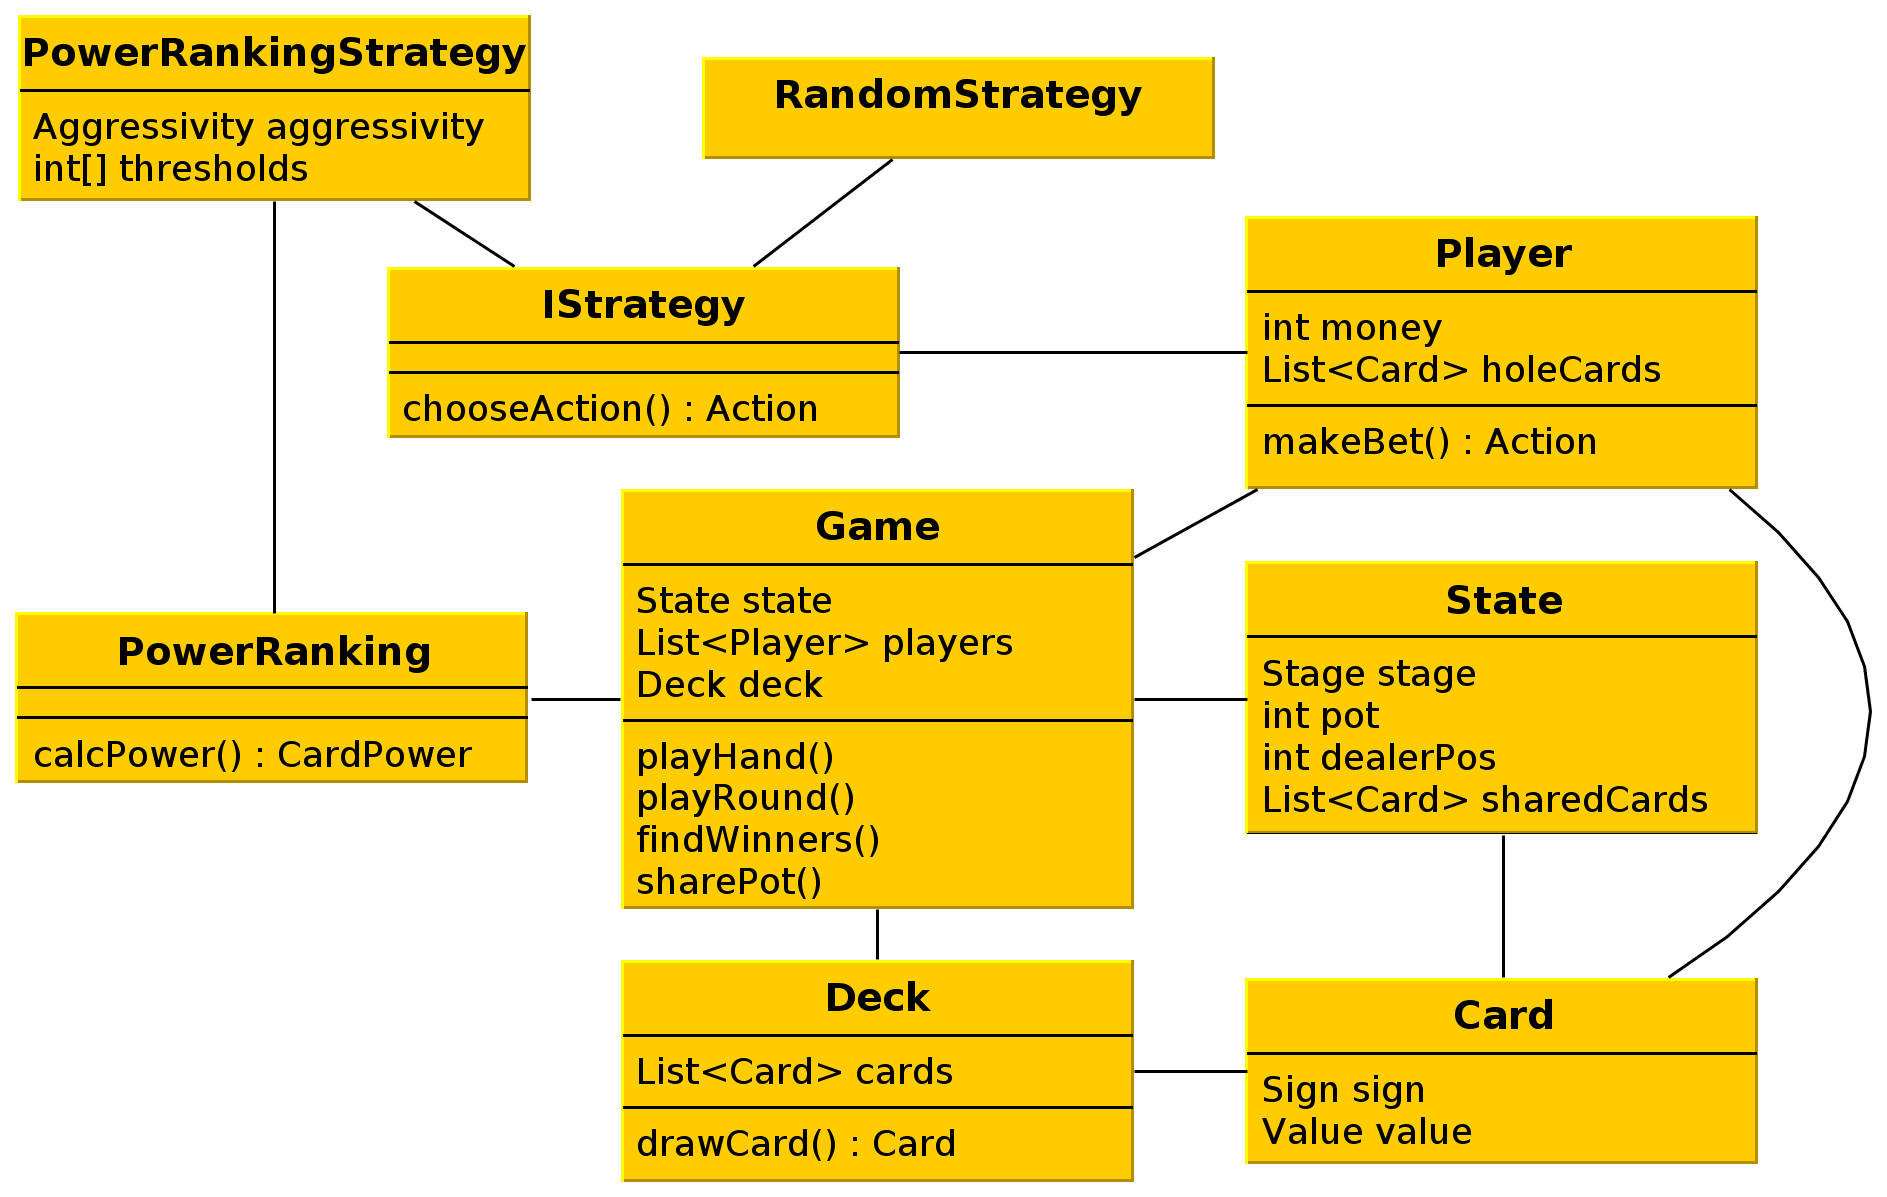
\includegraphics[width=0.8\textwidth]{images/phase1}
  \caption{Software design of phase I}
  \label{fig:phase1}
\end{figure}

\section{Strategies}
\label{sec:strategies}
In order to check the correctness of the game engine a \emph{Random Strategy} is implemented. The next step is to implement a more intelligent strategy that makes its decision on the basis of its current card power.

\subsection{Random Strategy}
\emph{Random Strategy} is the most simple strategy. It has no intelligence at all and chooses its decisions randomly. Firstly it makes a choise between \emph{Fold}, \emph{Call} and \emph{Raise}. In the case of \emph{Raise} the raise amount is calculated randomly between the onefold and the fourfold of the \emph{Big Blind}.

\subsection{Power-Ranking Strategy}
The action which the \emph{Power-Ranking Strategy} chooses depends on his current card power. If the card power reaches defined thresholds the player is calling or raising. Additionally there are three different levels of aggressivity. The thresholds for each aggressivity level are shown in the table \ref{tbl:powerRankingAggros}

\begin{table}[h]
	\centering
	\begin{tabular}[h]{l|l|l|l}
		\textbf{Aggressivity} & \textbf{Fold} & \textbf{Call} & \textbf{Raise}\\
		\hline
		Conservative & < three of a kind & >= three of a kind & >= straight\\
		Moderate & < two pairs & >= two pairs & >= three of a kind\\
		Risky & < one pair & >= one pair & >= two pairs\\
	\end{tabular}
	\label{tbl:powerRankingAggros}
	\caption{Thresholds for each aggressivity level}
\end{table}

Once the decision to raise is made, the amount to raise $r$ is calculated on the basis of the card power $p$, the aggressivity level $a$ and the size the big blind $b$ with the formula \ref{equ:powerranking}. The card power is a sequence of numbers where the first number indicates the hand category. $p = 8$ stands for a \emph{Straight Flush} and $p = 0$ stands for \emph{High Card}. The further numbers are needed to break a tie in the same category. The aggressivity level lies in between 1 and 2 where $a = 1$ stands for a conservative player, $a = 2$ for a moderate player and $a = 3$ for a risky player.

\begin{equation}
	\label{equ:powerranking}
	r = e^{(\frac{p}{3} - 3)} * 100 * a + b
\end{equation}

Since there are only 2 cards known during the pre-flop and the hand power can't be calculated the player acts like the player with the random strategy in this stage.

\section{Results}
Table \ref{tbl:resultsPhase1} shows five 10,000 hand runs where one unintelligent \emph{Random Strategy}-player competes with three \emph{Power-Ranking Strategy}-players.
\begin{table}[h]
	\centering
	\begin{tabular}[h]{l|r|r|r|r|r}
		& \textbf{Game 1} & \textbf{Game 2} & \textbf{Game 3} & \textbf{Game 4} & \textbf{Game 5}\\
		\hline
		Random & -34116 & -34456 & -32395 & -30322 & -35032\\
		Power Ranking (risky) & -6298 & -122 & 6552 & -2533 & -9379\\
		Power Ranking (moderate) & 34263 & 27587 & 24984 & 22343 & 25677\\
		Power Ranking (conservative) & 6054 & 6897 & 767 & 10423 & 18642\\
	\end{tabular}
	\label{tbl:resultsPhase1}
	\caption{Results of phase I}
\end{table}

As expected, the unintelligent random player loses bottomlessly. The player who dominates the game is the moderate \emph{Power-Ranking Strategy}-player. The thresholds at which he folds/calls/raises seem to be the most reasonable ones.

